\documentclass{article}

\usepackage[utf8]{inputenc}
\usepackage[T1]{fontenc}
\usepackage[francais]{babel}
\usepackage{titling}
\setlength{\droptitle}{-3cm}
\usepackage{graphicx}
\usepackage{underscore}
\usepackage{hyperref} 


\title{Compte rendu : Jour 1}
\author{CAROT Axel, ARISOY Ivan Can, \\ BREILLAD Matis, BELKHITER Medhi}
\date{\today}

\begin{document}
\maketitle

\section{Réunion avec les commanditaires}
Nous avons commencé notre journée par une réunion avec nos commanditaires pour bien comprendre les attentes du projet. Cette réunion nous a permis d'intégrer en quoi les solutions que nous devons proposer peuvent impacter les décisions prises en termes de politique. Les commanditaires ont aussi insisté sur la nécessité de disposer d'un outil intuitif et interactif.

\subsection{Compréhension du projet}
Dans le cadre du schéma de la solidarité territoriale, notre collaboration avec le département de l’Aude vise à doter les territoires des outils nécessaires pour valoriser leur potentiel. \\

Pour cela, nous développerons un indicateur composite ainsi qu’un outil d’aide à la décision. Cet outil interactif de visualisation de données doit être le plus intuitif possible facilitant ainsi son utilisation par les décideurs locaux. \\

Pour répondre à ces problématiques, nous disposons d’un jeu de données composé de plusieurs variables (16 indicateurs) concernant les communes du département de l’Aude. C’est à partir de ces indicateurs que nous construirons un indicateur composite qui permettra l'élaboration de politiques ciblées et efficaces.

\section{Travail effectué}

\subsection{ACP}
Nous disposons de 16 indicateurs que nous avons souhaité regrouper pour développer notre propre indicateur. Par exemple, nous pourrions créer une variable géographique unique englobant les temps d'accès aux collèges, à la bibliothèque et au chef-lieu (indicateurs 11, 12 et 13), ou une variable scolaire regroupant les informations sur le nombre de diplômés, de chômeurs et de cadres.\\

Pour ce faire, nous avons réalisé une analyse en composantes principales (ACP) afin de tenter de regrouper ces variables, mais sans obtenir de résultats convaincants. Les variables étant peu corrélées, comme le montre la matrice des corrélations, nous avons obtenu très peu d'informations pertinentes sur les deux principaux axes.

\vspace{2cm}
\begin{figure}[h]
    \centering
    \begin{minipage}{0.48\textwidth}
        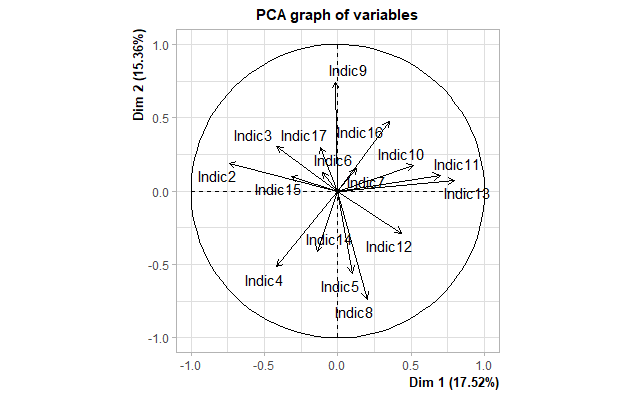
\includegraphics[width=\linewidth]{ACP_Na_sup.png}
        \caption{logo kaggle}
        \label{fig:kaggle1}
    \end{minipage}\hfill
    \begin{minipage}{0.48\textwidth}
        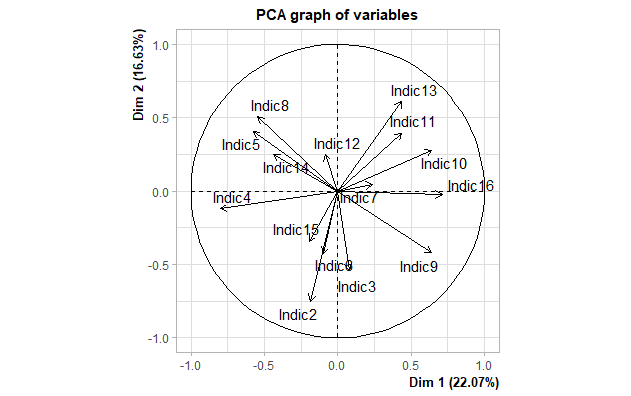
\includegraphics[width=\linewidth]{ACP_Moyenne.png}
        \caption{logo kaggle}
        \label{fig:kaggle2}
    \end{minipage}
\end{figure}

\begin{figure}[h]
    \centering
    \begin{minipage}{0.48\textwidth}
        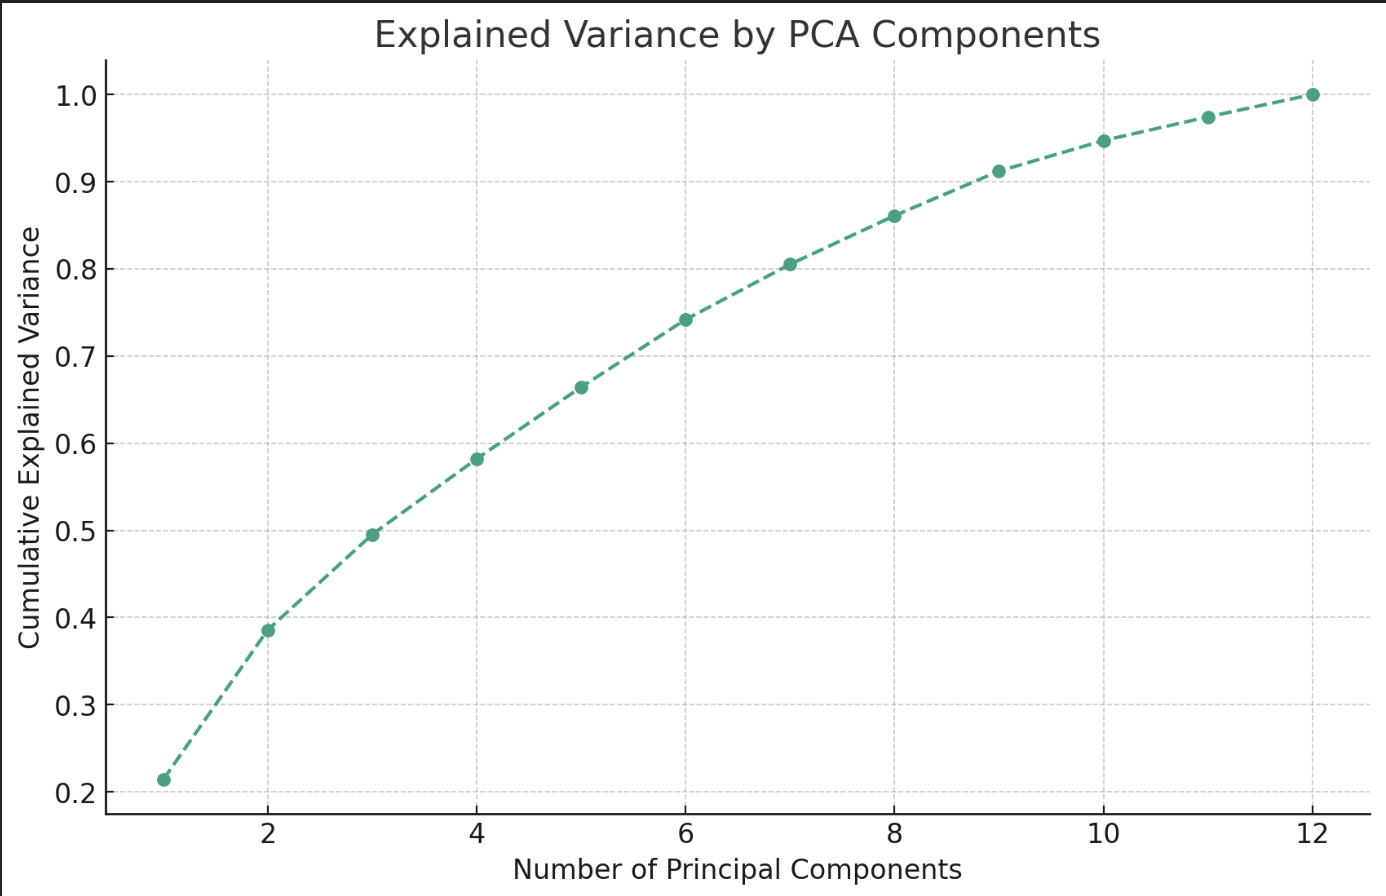
\includegraphics[width=\linewidth]{Screenshot_2024-03-04_at_18.00.52.png}
        \caption{logo kaggle}
        \label{fig:kaggle1}
    \end{minipage}\hfill
    \begin{minipage}{0.48\textwidth}
        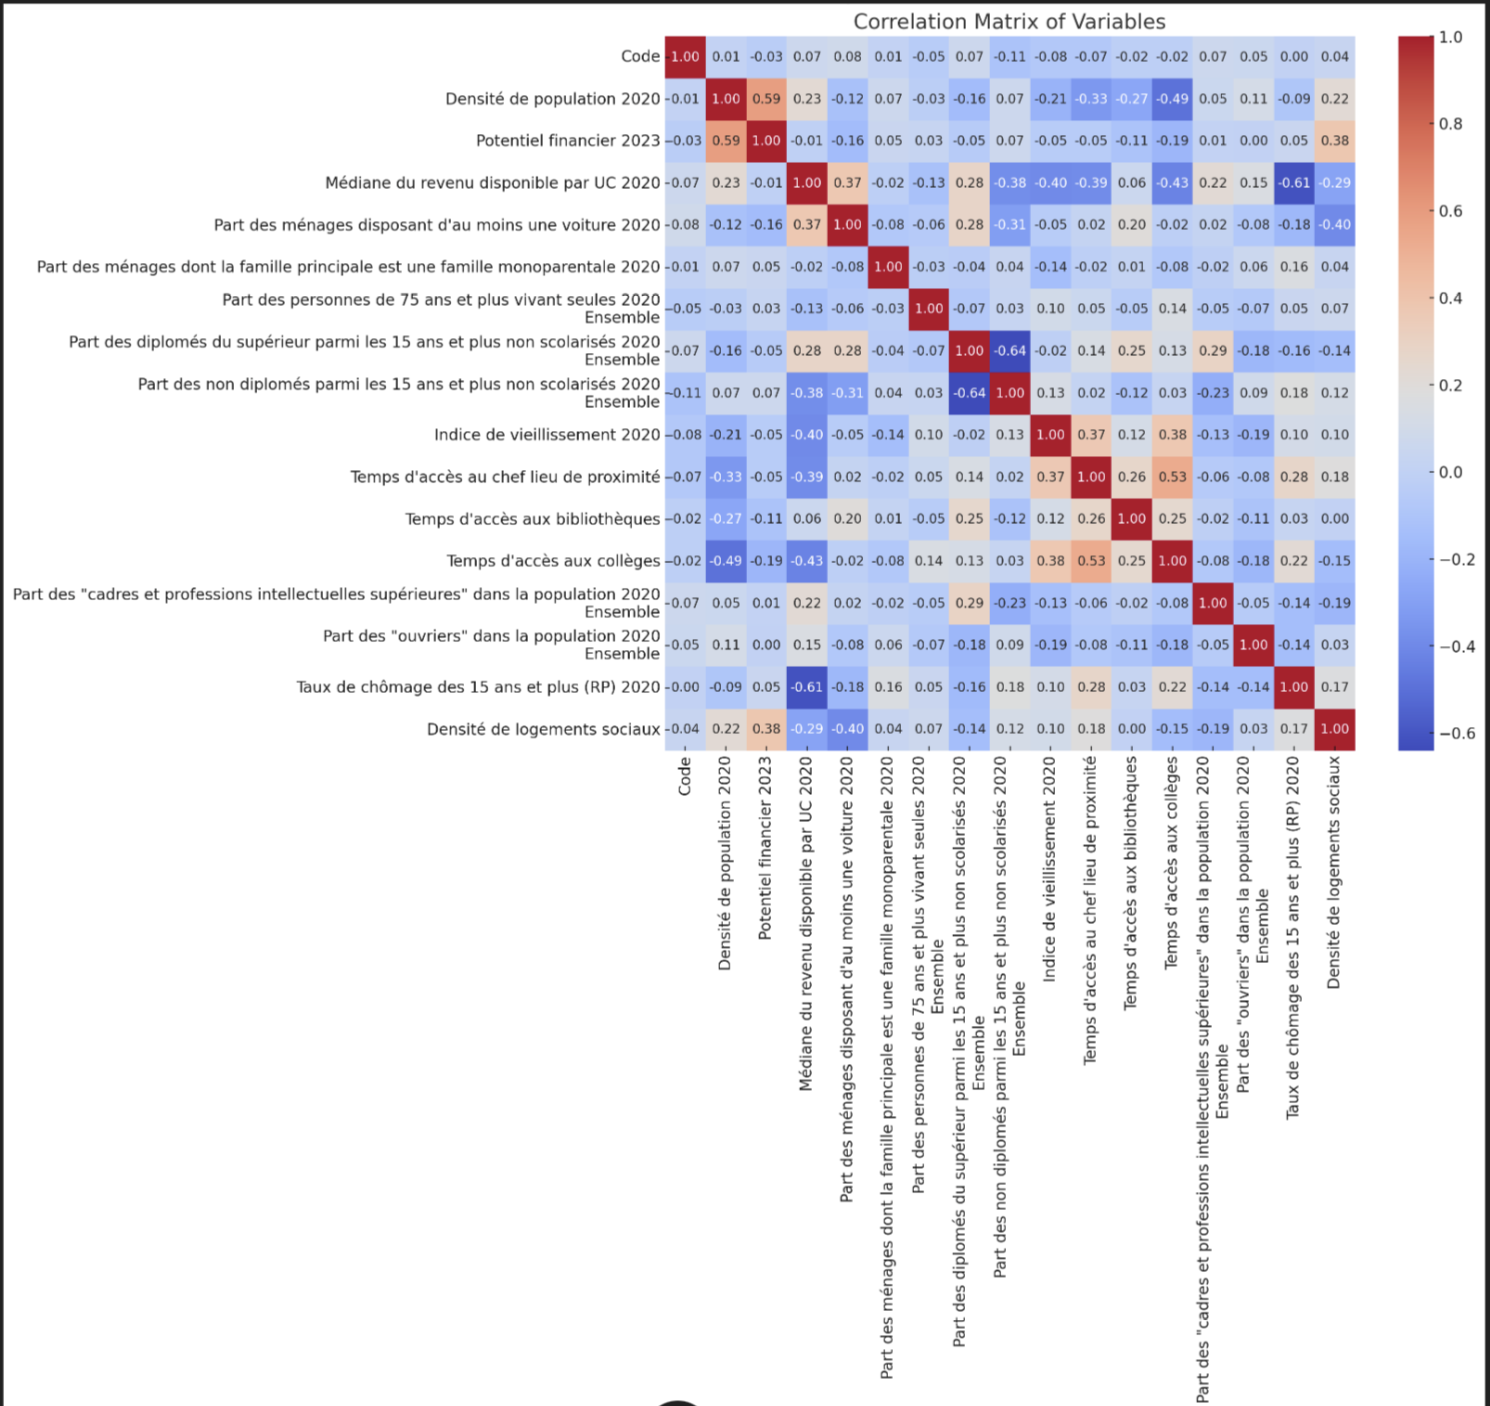
\includegraphics[width=\linewidth]{Screenshot_2024-03-04_at_17.59.59.png}
        \caption{logo kaggle}
        \label{fig:kaggle2}
    \end{minipage}
\end{figure}

De plus, il est important de noter la présence de nombreuses valeurs manquantes. Nous les avons remplacées par la moyenne des valeurs ou avons simplement supprimé les lignes concernées. Cependant, malgré ces ajustements, les résultats obtenus restent inchangés.

\subsection{Outil de visualisation de données}
Nous avons choisis de développer un outil de visualisation interactif inspiré du site : https://www.gapminder.org

\begin{figure}[h]
    \centering
    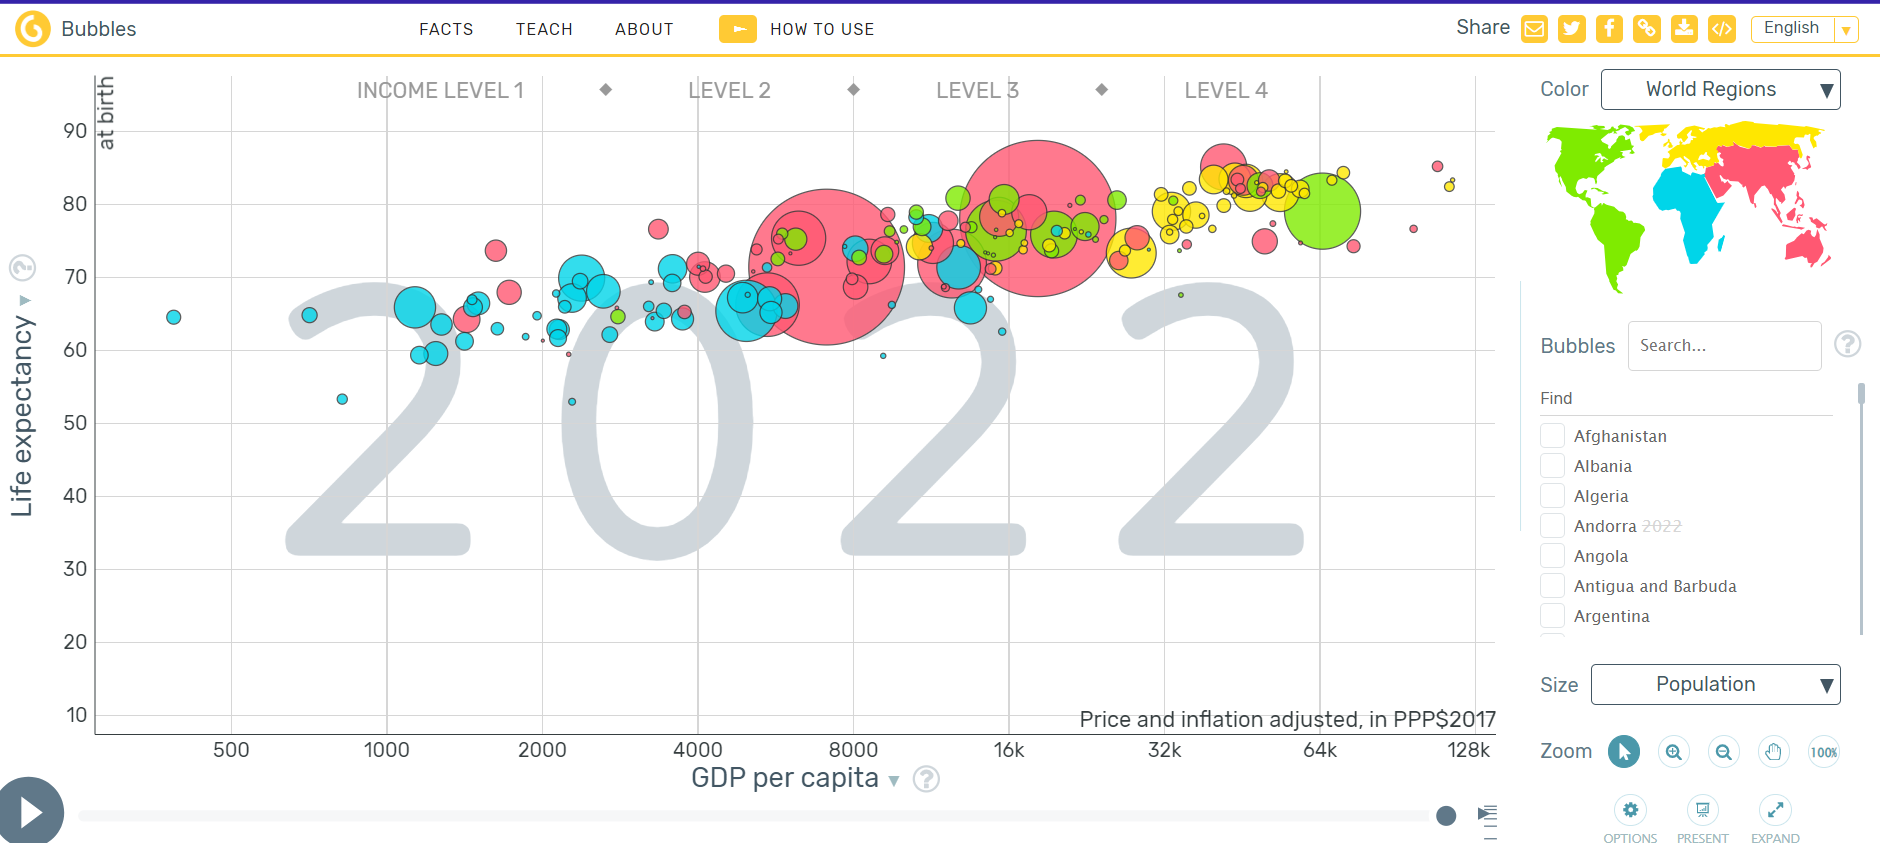
\includegraphics[width=1\textwidth]{gapminder_inspiration.png}
    \caption{logo kaggle}
    \label{fig:kaggle}
\end{figure}
\vspace{4cm}
Nous avons commencé par projeter les communes sans nous pencher sur les tailles des cercles ni sur leurs positions. L'objectif est de permettre de cliquer sur un cercle représentant une commune spécifique afin de visualiser les données la concernant sur un graphique en radar.

\begin{figure}[h]
    \centering
    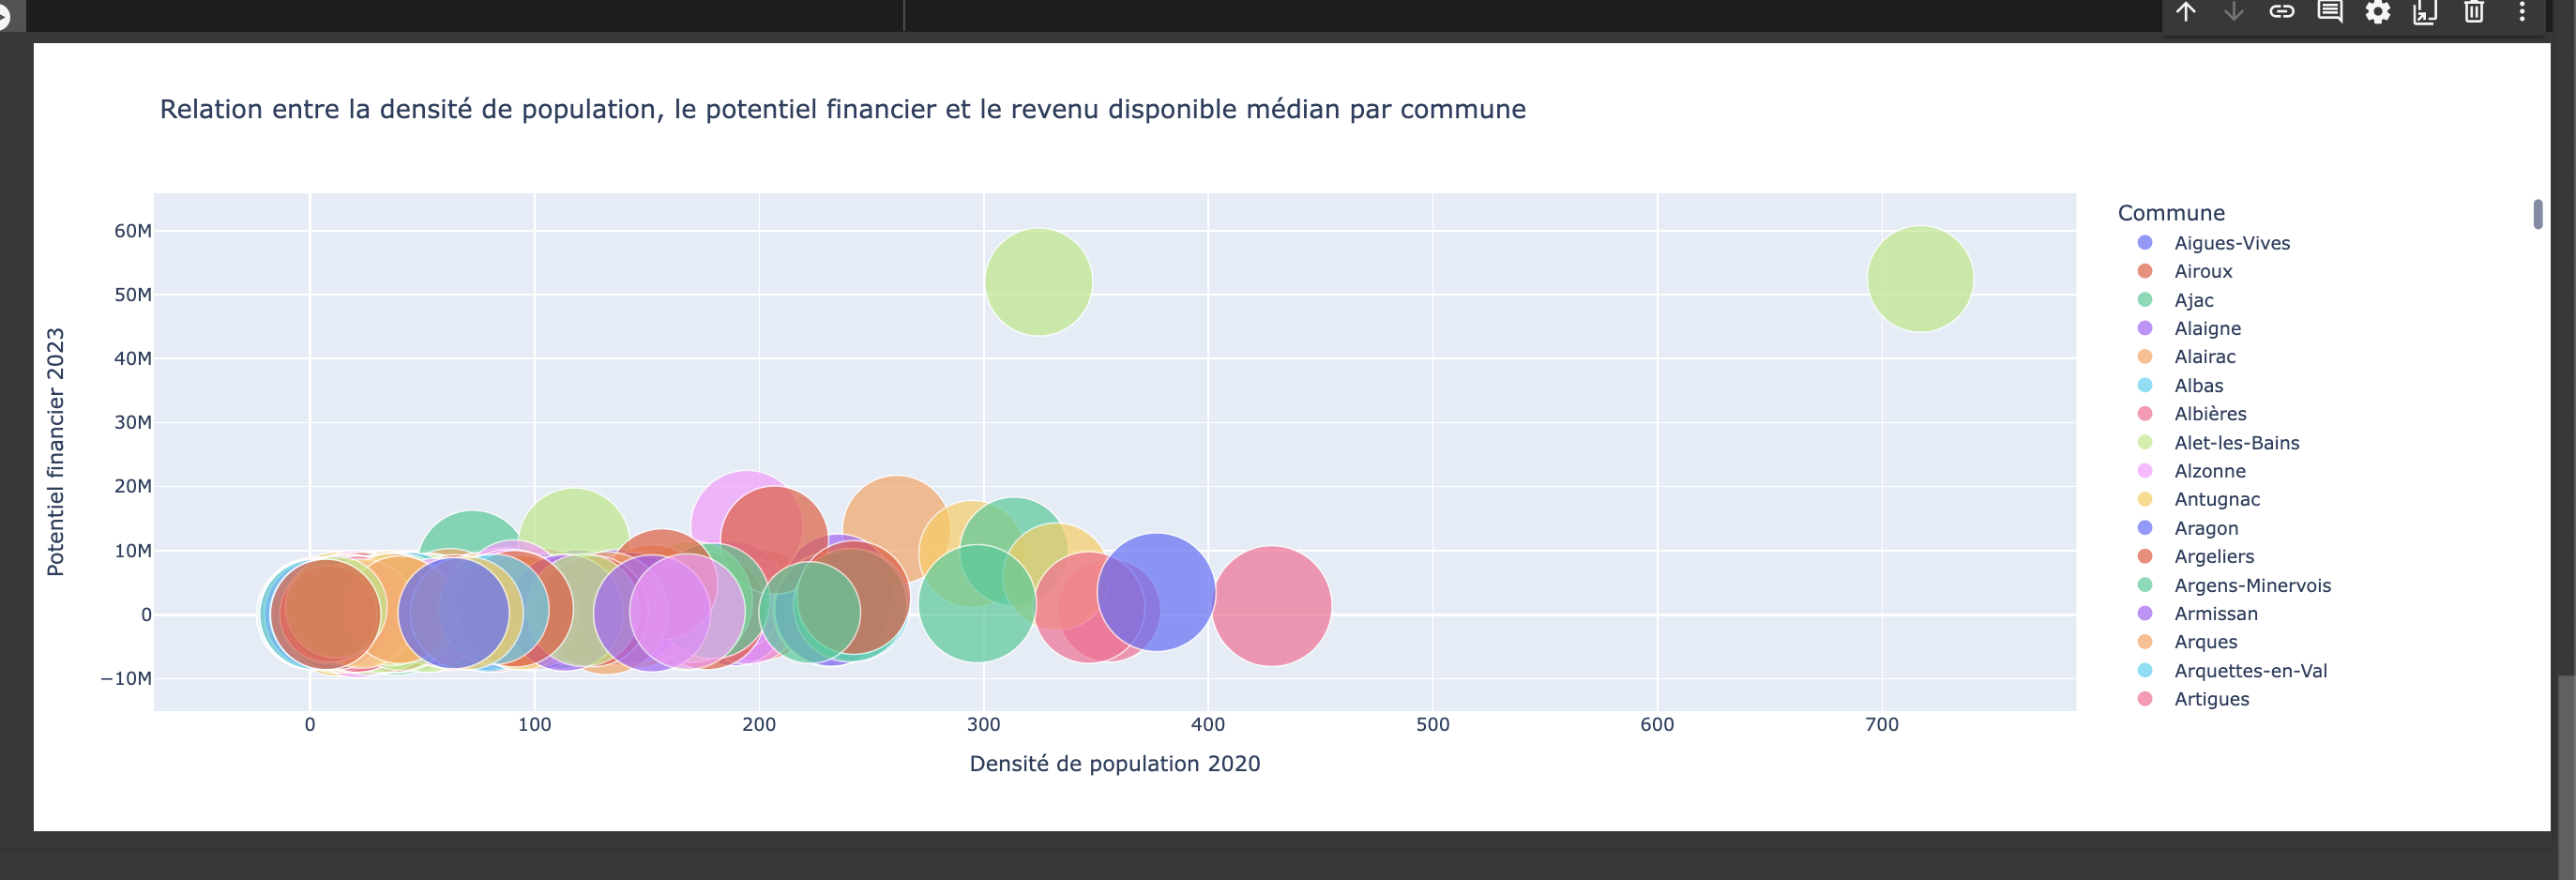
\includegraphics[width=1\textwidth]{Capture_decran_2024-03-04_a_18.02.42.png}
    \caption{logo kaggle}
    \label{fig:kaggle}
\end{figure}

\subsection{Radar plot}
Pour effectuer le radar plot, nous avons remplacé les valeurs manquantes par la moyenne en premier lieu. Puis, nous normalisé les données pour qu'elles soient uniformes. 
\begin{figure}[h]
    \centering
    \includegraphics[width=1\textwidth]{Capture d’écran 2024-03-04 à 19.34.45.png}
    \caption{logo kaggle}
    \label{fig:kaggle}
\end{figure}
\vspace{4cm}

\section{Travail à faire}
\begin{itemize}
    \item Finaliser le plot intéractif des cercles des communes et le radar plot.
    \item Réaliser un outil de visualisation de la distribution des variables.
    \item Développer l'indicateur.
    \item Réaliser un mode d'emploie de l'outil de Data viz.
\end{itemize} 

\section{Problèmes rencontrés}
Nous avons des problèmes liés aux données. Notamment le remplacement des données manquantes ainsi que la normalisation des données. 

\end{document}
